\documentclass[10pt,a4paper,ngerman]{article}

\usepackage[utf8]{inputenc}
\usepackage[T1]{fontenc}
\usepackage[safe,warn]{textcomp}
\usepackage{tgtermes}
\usepackage[scaled]{berasans}
\renewcommand*\ttdefault{txtt}
\usepackage{pdfpages}

\usepackage{babel}

\usepackage{amsmath}
\usepackage{amsfonts}
\usepackage{amssymb}

\usepackage{listings}

\usepackage{geometry}
\geometry{left=25mm,right=2cm, top=2cm, bottom=2cm}

\usepackage{fancyhdr}
\pagestyle{fancy}
\fancyhf{}
\fancyhead[L]{Universität zu Lübeck, \texttt{getRandomNumber()\{return 4;\}}}
\fancyhead[R]{\thepage}
\renewcommand{\headrulewidth}{0.4pt}

\title{Team Contest Reference\\ \texttt{getRandomNumber()\{return 4;\}}}
\author{Universität zu Lübeck}
\begin{document}
\lstset{basicstyle=\ttfamily\footnotesize,numbers=left,numberstyle=\tiny,tabsize=2,numbersep=5pt}
\maketitle\thispagestyle{fancy}

\tableofcontents

\section{Mathematische Algorithmen}
\subsection{Primzahlen}
Für Primzahlen gilt immer (aber nicht nur für Primzahlen)
\[a^p\equiv a\mod p \quad\text{ bzw. }\quad a^{p-1}\equiv 1 \mod p.\]
\subsubsection{Sieb des Eratosthenes}
\lstinputlisting[language=Java]{eratosthenes.java}
\subsubsection{Primzahlentest}
\lstinputlisting[language=Java]{isprim.java}
\subsection{Binomial Koeffizient}
\lstinputlisting[language=Java]{binomial.java}
\subsection{Modulare Arithmetik}
Bedeutung der größten gemeinsamen Teiler:
\[ d = \text{ggT}(a,b) = as+bt \]
Verwendung zu Berechnung des inversen Elements $b$ zu $a$ bezüglich einer Restklassengruppe $n$ ($a$ und $n$ müssen teilerfremd sein):
\[ ab\equiv 1 \mod n\quad\Leftrightarrow\quad s\equiv b \mod n\quad\text{ für }1=\text{ggT}(a,n)\]
\subsubsection{Erweiterter Euklidischer Algorithmus}
\lstinputlisting[language=Java]{eea.java}
\subsection{Matrixmultiplikation}
Strassen-Algorithmus: $\mathbf{C} = \mathbf{A} \mathbf{B} \qquad \mathbf{A},\mathbf{B},\mathbf{C} \in R^{2^n \times 2^n}$
\begin{eqnarray*}
\mathbf{C}_{1,1} & =& \mathbf{A}_{1,1} \mathbf{B}_{1,1} + \mathbf{A}_{1,2} \mathbf{B}_{2,1} \\
\mathbf{C}_{1,2} &=& \mathbf{A}_{1,1} \mathbf{B}_{1,2} + \mathbf{A}_{1,2} \mathbf{B}_{2,2}\\
\mathbf{C}_{2,1} &=& \mathbf{A}_{2,1} \mathbf{B}_{1,1} + \mathbf{A}_{2,2} \mathbf{B}_{2,1} \\
\mathbf{C}_{2,2} &=& \mathbf{A}_{2,1} \mathbf{B}_{1,2} + \mathbf{A}_{2,2} \mathbf{B}_{2,2}
\end{eqnarray*}
\section{Datenstukturen}
\subsection{Fenwick Tree (Binary Indexed Tree)}
\lstinputlisting[language=Java]{fenwick.java}

\section{Graphenalgorithmen}
\subsection{Topologische Sortierung}
\lstinputlisting[language=Java]{toposort.java}
\subsection{Prim (Minimum Spanning Tree)}
\lstinputlisting[language=c]{prim.c}
\subsection{Maximaler Fluss (Ford-Fulkerson)}
\lstinputlisting[language=c]{ford-fulkerson.c}
\lstinputlisting[language=java]{ford-fulkerson.java}
\subsection{Floyd-Warshall}
\lstinputlisting[language=java]{floyd.java}
\subsection{Dijkstra}
\lstinputlisting[]{dijkstra.txt}

\section{Geometrische Algorithmen}
\subsection{Graham Scan (Convex Hull)}
\lstinputlisting[language=java]{graham.java}
\subsection{Maximum Distance in a Point Set}
\lstinputlisting[language=java]{maxdist.java}
\subsection{Punkt in Polygon}
\lstinputlisting[language=java]{PointInPoly.java}
\section{Verschiedenes}
\subsection{Potenzmenge}
\lstinputlisting[language=java]{powerset.java}
\subsection{Longest Common Subsequence}
\lstinputlisting[language=c]{longest_common_subsequence.c}
\subsection{Longest Increasing Subsequence}
\lstinputlisting[language=c]{longest_increasing_subsequence.c}
\section{Eine kleine C-Referenz}

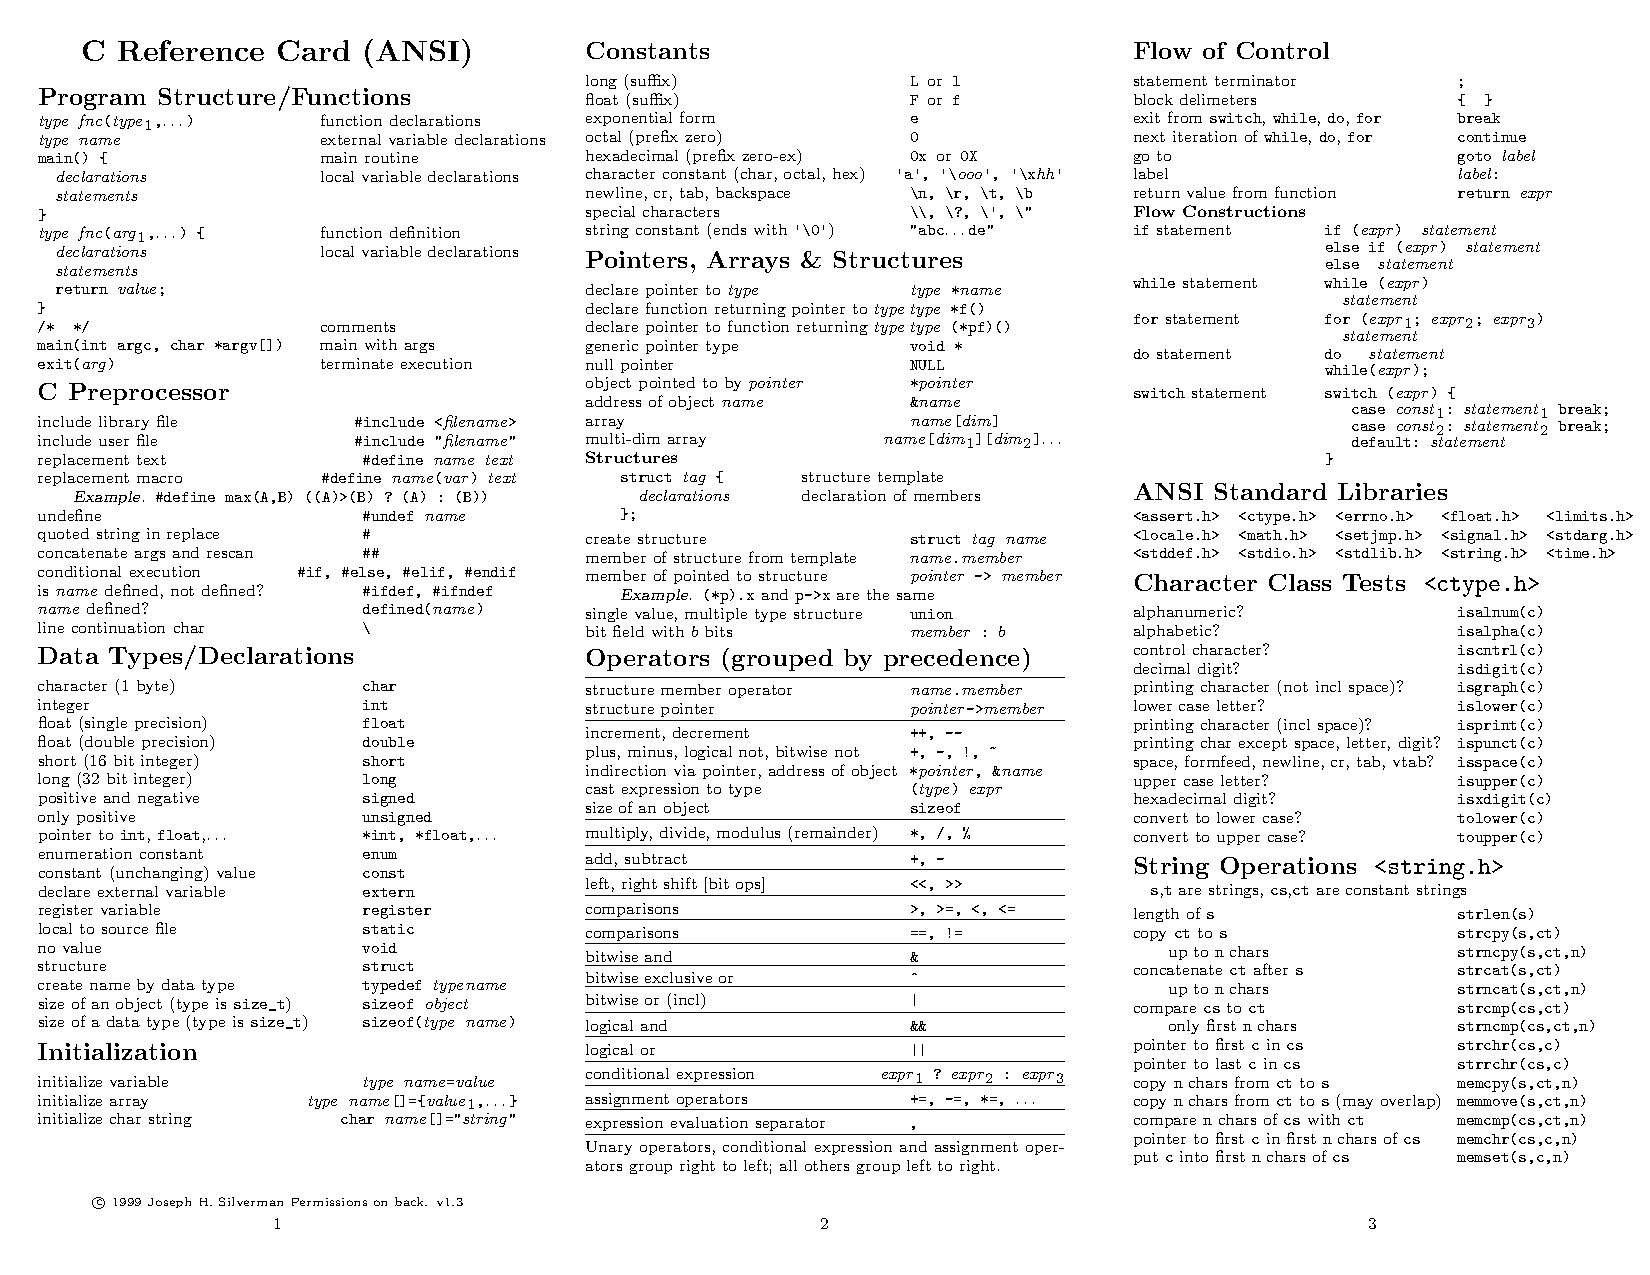
\includepdf[
	scale=0.9,
	angle=90,
	pages=1,
	pagecommand={		
}]{c-refcard.pdf}

\includepdf[
	scale=0.9,
	angle=90,
	pages=2,
	pagecommand={		
}]{c-refcard.pdf}


\end{document}